\section{RQ3: Repository-Aware Analysis}

To answer \roundframe{RQ3}, we analyze whether skills flagged as malicious by automated scanners remain suspicious when evaluated within the context of their surrounding GitHub repositories. Existing scanners typically analyze skills in isolation, which can lead to false positives when benign functionality appears suspicious without considering the broader context. 
Our analysis shows that repository context plays an important role, as many flagged skills reside in repositories whose documentation and codebase align with the skill functionality and do not exhibit malicious behavior. We focus on skills that are flagged as malicious by both the Cisco Skill Scanner (severity high or critical) and our GPT-5.3-based analyzer with a score greater than 3, resulting in 8,153 flagged (skill, repository) combinations. We exclude two instances from our analysis. First, we exclude ClawHub skills, as no GitHub repository context exists. Second, we exclude skills located in the repository root, as this setup only allows metadata based analysis but not codebase scoring. Among the skills, we find only $\sim$100 hosted as standalone GitHub repositories.  From the remaining set of skill and repository, we randomly sample 3,000 skill repository combinations and collect the corresponding repository metadata together with full repository (failed in 113 cases) clones.


\paragraph{Metadata Score.}

To understand the repository context of flagged skills, we analyze repository metadata such as size, age, activity, popularity (stars and forks), and issue activity using predefined bucket ranges. \Cref{fig:metadata_buckets} shows the distribution of these metadata scores for the 1,431 repositories containing flagged skills. Overall, these repositories tend to be small and have limited popularity. Almost half of the repositories (47.6\%) are smaller than 2\,MB, while only 11.1\% exceed 50\,MB. Popularity signals are generally low. 43.4\% of repositories have no stars and 66.5\% have no forks, and none of the repositories exceed 100 stars or forks. Similarly, 64.0\% of repositories have no open issues. Most repositories are relatively young and moderately maintained. The majority (73.0\%) were created between two weeks and four months before the crawl, while 17.1\% are older than one year. Despite their limited popularity, many repositories remain active: 47.4\% were updated within the last week. To evaluate whether repositories with flagged skills differ from typical skill repositories, we repeat the analysis using a random set of 1,500 repositories with a matching marketplace distribution. The resulting distributions are similar, suggesting that repositories containing flagged skills do not exhibit distinct metadata characteristics. Instead, the observed differences are driven by marketplace composition rather than the presence of suspicious skills.
Repositories originating from SkillsDirectory achieve higher metadata scores, which reflects more established projects, whereas Skills.sh and GitHub Archive repositories exhibit lower scores, which correlates with the lack of moderation for hosted skills.

\begin{figure}[t]
  \centering
  \begin{minipage}{0.95\linewidth}
      \centering
    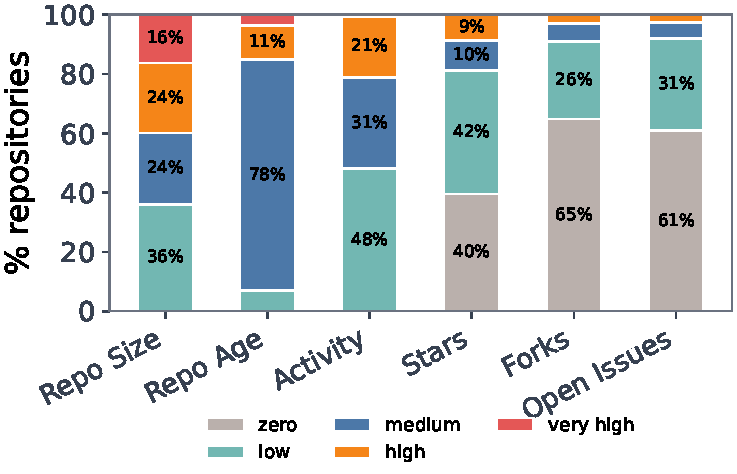
\includegraphics[width=0.89\linewidth]{figures/metadata_score_categories.pdf}
    \caption{Metadata scores for unique repositories.}
    \Description{The figure presents the metadata scores for unique repositories.}
    \label{fig:metadata_buckets}
  \end{minipage}
  
  \end{figure}

  
\paragraph{Codebase Score.}
To evaluate whether a flagged skill aligns with its surrounding repository context, we design an evidence-based prompt that assesses the relationship between the skill and the repository codebase. The evaluation considers domain alignment, code similarity, README consistency, repository support signals, and a maliciousness-adjusted score. To control analysis cost, we limit the repository context to up to 200 lines from the SKILL.md and README files and up to three repository files (100 lines each). Most repositories provide sufficient context for evaluation. Among the analyzed repositories, 94.1\% contain a README and 65.7\% contain repository code, with 61.9\% containing both. Repository context frequently aligns with the skill purpose. Domain matching is high for 45.9\% of skills and medium for 26.1\%, indicating that roughly 72\% of repositories exhibit at least moderate thematic alignment with the skill description. Direct code alignment is less common, with 9.9\% showing high similarity and 28.6\% medium similarity. Importantly, very few repositories exhibit malicious repository-level behavior. 98.0\% of repositories fall into the lowest maliciousness category, with only two repositories showing high maliciousness signals. Security-tooling related signals appear in a small subset of repositories (5.2\%). These results suggest that the majority of flagged skills are embedded in repositories whose documentation and structure are broadly consistent with the skill purpose, providing strong contextual evidence that many scanner alerts represent false positives.


\begin{figure}[t]
    \centering
    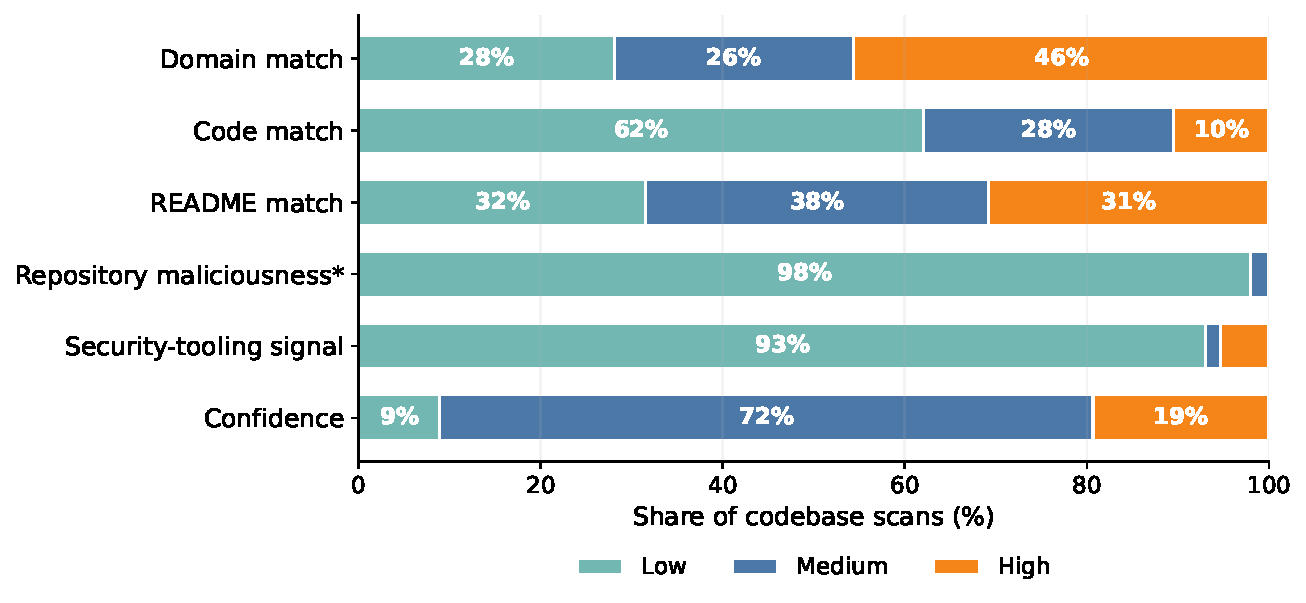
\includegraphics[width=0.95\linewidth]{figures/codebase_score_categories.pdf}
    \caption{Codebase score category results, marked with * means lower is better.}
    \Description{The figure shows the codebase score results per category.}
    \label{fig:codebase_categories}
\end{figure}

\iffalse
\paragraph{Economic Feasibility.}
We evaluate the cost of repository-context analysis using a sample of 20 skill–repository pairs. On average, each analysis consumes 6,725 input tokens and 125 output tokens. Using the current GPT-5 pricing model (\$1.25 per million input tokens and \$10 per million output tokens), a single analysis costs approximately \$0.0097 without caching. With prompt caching enabled, the cost drops to roughly \$0.0021 per analysis.
Applying this approach to the full sample of 3,000 skills resulted in a total cost of approximately \$24, including occasional retries. While continuous daily scans of the entire ecosystem would remain expensive, periodic scans (e.g., weekly) are economically feasible for skill marketplaces such as SkillsDirectory.
\fi


\paragraph{Repository Context Score.}
\Cref{fig:score_panel} shows the distribution of repositories across the individual scoring components. The distributions reflect an important observation: the majority of repositories in which skills reside were flagged as non-malicious. This is particularly visible in the codebase score, which already assigns a baseline score of 40 when a repository is classified as non-malicious. Consequently, the codebase score distribution spans a wide range, with a mean of 65.1 and values extending up to 97, reflecting varying degrees of alignment between the skill implementation and the surrounding repository code. Only a small fraction of repositories achieves near-perfect alignment, with most scores distributed between 40 and 70.
In contrast, the metadata score is lower and more compressed, with a mean of 42.9. A large number of repositories created within the past six months. As the ecosystem matures and more skills become embedded in established and actively maintained codebases, this component will likely increase. The current distribution reflects the early stage of the skill ecosystem. The repository-context score, which combines both signals, yields a smoother distribution, with a mean of 58.5 and no significant outliers. Most repositories already reach moderate trust levels, primarily driven by the codebase analysis, which evaluates alignment between the skill and the surrounding code. Overall, this combined scoring approach allows us to contextualize the large number of initially flagged skills.

\begin{figure}[t]
    \centering
    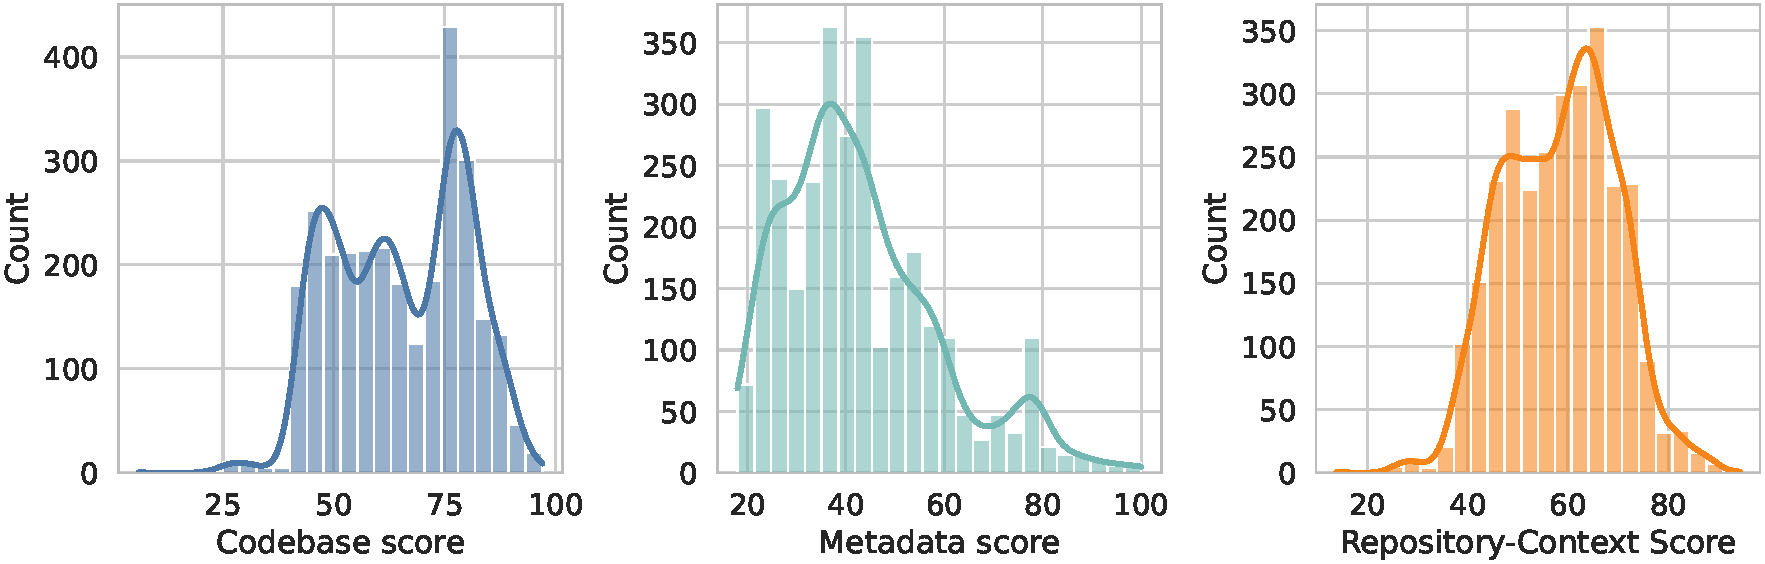
\includegraphics[width=\linewidth]{figures/score_panel.pdf}
    \caption{Repository context score and its weighted subcomponents, with 70\% codebase score and 30\% metadata score.}
    \Description{The figure illustrates the repository context score together with its weighted subcomponents.}
    \label{fig:score_panel}
\end{figure}


\paragraph{Score Interpretation.}
The repository-context score combines the codebase score (70\%) and the repository metadata score (30\%). As shown in \Cref{fig:score_panel}, the resulting distribution is relatively
smooth (mean 58.5) and does not exhibit significant outliers. Most repositories already reach moderate trust levels, primarily driven by the codebase analysis, which evaluates structural
alignment between the skill and the surrounding code and is largely independent of repository age. To help interpret this metric, we divide the repository-context score into three
categories. The lowest category ($<40$) represents skills that appear weakly embedded in their repository context or originate from repositories with low maturity. This group contains 121
cases (4.2\%) with an average context score of 36.2.
The majority of skills fall into the intermediate category ($40$–$<60$), representing skills that are connected to a repository but whose surrounding context provides only moderate
support. This group includes 1,373 cases (47.6\%) with an average context score of 50.8.
Finally, 1,393 skills (48.3\%) fall into the highest category ($\geq60$), indicating strong alignment between the skill and the repository codebase and documentation. In this group, the
average codebase score reaches 77.2, suggesting that the repository content strongly supports the intended functionality of the skill.
Overall, only a small fraction of flagged skills (4.2\%) appear poorly embedded in their repository context, while the vast majority show moderate to strong alignment with their
surrounding repositories.


\paragraph{Suspicious Repositories.}
We identify a small subset of repositories where the skill is aligned with the codebase but the repository itself appears suspicious and is not categorized as a security tool. In total 15 cases fall into this category. This corresponds to 0.52\% of the 2,887 skill-repository combinations with API/codebase evaluation. While the metadata score differs only slightly (mean 41.1 vs.\ 42.9), these repositories show substantially lower codebase scores (51.5 vs.\ 65.2). Consequently, their repository-context score is also lower (48.4 vs.\ 58.5), indicating that the combined scoring effectively reacts to suspicious environments and separates them from the rest of the ecosystem.

\paragraph{Cross-Repository Scores.}
To understand whether repository context influences the evaluation of individual skills, we analyze skills that appear in multiple repositories. In total, 354 skills appear in more than one repository. Across these skills, the median cross repository variance of the codebase score is 42.0, which corresponds to a median standard deviation of 6.48 and a median score range of 15.0 points. These results indicate moderate context sensitivity, where the same skill can receive noticeably different scores depending on the surrounding repository. The distribution also exhibits a substantial tail of highly variable skills, where the 90th percentile range reaches 33.75 score points. This observation suggests that repository context can significantly influence how a system interprets a skill's behavior.

\paragraph{Score Validation.}
Currently, no publicly available dataset exists that labels repositories as malicious with respect to agent skills. Instead, we follow an inverse validation approach: we evaluate whether repositories containing scanner-flagged skills appear benign when inspected manually and whether our repository-aware scoring reflects these observations.
To obtain qualitative validation, we randomly sample 20 repositories from the flagged set and provide them to two independent researchers for manual assessment. Reviewers were asked to determine whether the repository appeared benign or suspicious based on its documentation, code structure, and functionality. Both reviewers classified all 18 reviewed repositories as benign, the two remaining were not available anymore. This indicates that the repositories themselves do not exhibit obvious malicious intent.

Reviewers also assessed repository maturity. In this case, judgments were more heterogeneous: Reviewer~1 classified 5/18 repositories with medium maturity, and 1/18 as high, while Reviewer~2 classified maturity as medium for 14/18 and 3/18 high. The two reviewers agreed on maturity in 5 of the 18 comparable cases. 
In \Cref{fig:maturity_validation}, we compare manual scores, computed as the average score of both reviewers, with the scores produced by our analysis. Overall, the figure reveals a positive correlation, as higher maturity scores assigned by the metadata score coincide with higher scores from human reviewers.
Overall, the manual review supports our repository-aware scoring approach: repositories containing scanner-flagged skills generally appear benign, even under manual expert review, while manual maturity assessments match the automatically calculated metadata score. 

\begin{figure}[t]
    \centering
    \includegraphics[width=1\linewidth]{figures/maturity_validation.pdf}
    \caption{Comparison of maturity scores assigned by manual reviewers and our repository aware scoring approach.}
    \Description{The figure compares maturity scores assigned by manual reviewers with those produced by our repository-aware scoring approach.}
    \label{fig:maturity_validation}
\end{figure}

